\textit{Dans tout cet exercice, les probabilités seront arrondies, si nécessaire, à $10^{-3}$.}

\medskip

D’après une étude, les utilisateurs réguliers de transports en commun représentent 17\,\% de la population française. Parmi ces utilisateurs réguliers, 32\,\% sont des jeunes âgés de 18 à 24 ans.

\hfill~(Source : TNS-Sofres)

\medskip

\textbf{Partie A :}

\medskip

On interroge une personne au hasard et on note :
\begin{itemize}
	\item R l’événement : « La personne interrogée utilise régulièrement les transports en commun » ;
	\item J l’événement : « La personne interrogée est âgée de 18 à 24 ans ».
\end{itemize}

\begin{enumerate}
	\item Représentez la situation à l’aide de cet arbre pondéré, que vous recopierez sur
	votre copie, en y reportant les données de l’énoncé.
	\begin{center}
		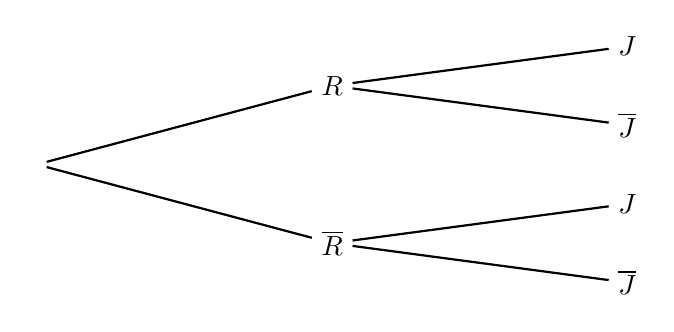
\begin{tikzpicture}[xscale=1,yscale=1]
			\tikzstyle{fleche}=[thick]
			\tikzstyle{feuille}=[]
			\def\DistanceInterNiveaux{3}
			\def\DistanceInterFeuilles{1}
			\def\NiveauA{(0)*\DistanceInterNiveaux}
			\def\NiveauB{(1.25)*\DistanceInterNiveaux}
			\def\NiveauC{(2.5)*\DistanceInterNiveaux}
			\def\InterFeuilles{(-1)*\DistanceInterFeuilles}
			\node[feuille] (R) at ({\NiveauA},{(1.5)*\InterFeuilles}) {$ $};
			\node[feuille] (Ra) at ({\NiveauB},{(0.5)*\InterFeuilles}) {$R$};
			\node[feuille] (Raa) at ({\NiveauC},{(0)*\InterFeuilles}) {$J$};
			\node[feuille] (Rab) at ({\NiveauC},{(1)*\InterFeuilles}) {$\overline{J}$};
			\node[feuille] (Rb) at ({\NiveauB},{(2.5)*\InterFeuilles}) {$\overline{R}$};
			\node[feuille] (Rba) at ({\NiveauC},{(2)*\InterFeuilles}) {$J$};
			\node[feuille] (Rbb) at ({\NiveauC},{(3)*\InterFeuilles}) {$\overline{J}$};
			\draw[fleche] (R)--(Ra) ;
			\draw[fleche] (Ra)--(Raa) ;
			\draw[fleche] (Ra)--(Rab) ;
			\draw[fleche] (R)--(Rb) ;
			\draw[fleche] (Rb)--(Rba) ;
			\draw[fleche] (Rb)--(Rbb) ;
		\end{tikzpicture}
	\end{center}
	\item Calculer la probabilité $P(R \cap J)$.
	\item D’après cette même étude, les jeunes de 18 à 24 ans représentent 11\,\% de la
	population française.
	
	Montrer que la probabilité que la personne interrogée soit un jeune de 18 à 24 ans n’utilisant pas régulièrement les transports en commun est $0,056$ à $10^{-3}$.
	\item En déduire la proportion de jeunes de 18 à 24 ans parmi les utilisateurs non réguliers des transports en commun.
\end{enumerate}

\medskip

\textbf{Partie B :}

\medskip

Lors d’un recensement sur la population française, un recenseur interroge au hasard 50 personnes en une journée sur leur pratique des transports en commun.

La population française est suffisamment importante pour assimiler ce recensement
à un tirage avec remise.

\smallskip

Soit $X$ la variable aléatoire dénombrant les personnes utilisant régulièrement les transports en commun parmi les 50 personnes interrogées.

\begin{enumerate}
	\item Déterminer, en justifiant, la loi de $X$ et préciser ses paramètres.
	\item Calculer $P(X=5)$ et interpréter le résultat.
	\item Le recenseur indique qu’il y a plus de 95\,\% de chance pour que, parmi les 50 personnes interrogées, moins de 13 d’entre elles utilisent régulièrement les transports en commun.
	
	Cette affirmation est-elle vraie ? Justifier votre réponse.
	\item Quel est le nombre moyen de personnes utilisant régulièrement les transports en commun parmi les 50 personnes interrogées ?
\end{enumerate}

